%****************************************************************************%
%* DIET Programmer's Guide                                                  *%
%*                                                                          *%
%*  Author(s):                                                              *%
%*    - Philippe COMBES (Philippe.Combes@ens-lyon.fr)                       *%
%*                                                                          *%
%* $LICENSE$                                                                *%
%****************************************************************************%
%* $Id$
%* $Log$
%* Revision 1.11  2007/04/17 13:34:52  ycaniou
%* Error in debug.tex header
%* Removes some warnings during doc generation
%*
%* Revision 1.10  2007/02/16 10:27:35  ycaniou
%* Beginning of a chapter on the Diet debugging (here, valgrind).
%*
%* Revision 1.9  2006/11/16 14:09:19  eboix
%* - Programmers guide converted from autotools to cmake.
%* - cmake summary deported to Cmake sub-dir.   --- Injay2461
%*
%* Revision 1.8  2006/06/30 21:20:37  eboix
%*   Cmake and dart related modifications:
%*    - [c]cmake's ambiguous option DIET_MAINTAINER_MODE removed. Building the
%*      documentation is now only controled by DIET_BUILD_DOCUMENTATION (and
%*      user's, developpers and doxygen docs are handled together). In order
%*      to use the Maintainer build type add -DCMAKE_BUILD_TYPE:STRING=Maintainer
%*      as [c]cmake option.
%*    - Created Cmake/Dart subdir as placeholder for Dart related utilities.
%*    - Cmake/DashBoardScript.cmake renamed to Cmake/Dart/DashBoardScript.cmake
%*                                                                 --- Injay2461
%*
%* Revision 1.7  2006/01/25 17:26:04  pfrauenk
%* CoRI : Some useful information about CoRI now available
%*
%* Revision 1.6  2005/08/08 08:26:57  ycaniou
%* Fixed remaining reference to ../UserManual/fig/logo in ProgrammersGuide.tex to ./fig/logo
%* Addition of a cp of the ../UserManual/fig/logo in the makefile: now it compiles
%* Addition of a batch section (also contains general remarks which have to be dispatched if pertinent). Not complete!
%*
%* Revision 1.4  2004/01/09 15:26:53  cpera
%* Add Annexe on Autotools.
%*
%* Revision 1.3  2003/12/15 00:13:53  ecaron
%* New structure for the first sheet
%*
%* Revision 1.2  2003/09/17 14:41:28  pcombes
%* Split the .tex according to its chapters.
%*
%* Revision 1.1  2003/09/09 12:42:44  pcombes
%* Reorganization of doc: include CS in a programmer's guide.
%****************************************************************************%

\documentclass[11pt,a4paper]{report}
\makeatletter
%\makeatother
\usepackage{fancyheadings}
%\usepackage[french]{babel}
%\usepackage[latin1]{inputenc}
\usepackage{multicol}
\usepackage{verbatim}
\usepackage[headings]{fullpage}
\usepackage{url}

\usepackage{graphicx}
\graphicspath{{../UM/fig}}

\newsavebox{\logobox}
%\sbox{\logobox}{\includegraphics[scale=0.3]{../UsersManual/fig/logo_DIET.ps}}
\sbox{\logobox}{\includegraphics[scale=0.3]{fig/logo_DIET.ps}}
\newcommand{\logo}{\usebox{\logobox}}

%%%%
\renewcommand{\title}{DIET Programmer's Guide}
%%%%

\pagestyle{fancyplain}
\lhead[\fancyplain{\title}{\title}]
      {\fancyplain{\title}{\title}}
\chead{}
\rhead[\fancyplain{\logo}{\logo}]{\fancyplain{\logo}{\logo}}

\lfoot[\fancyplain{INRIA}{INRIA}]{\fancyplain{INRIA}{INRIA}}
\cfoot[\fancyplain{}{}]{\fancyplain{}{}}
\rfoot[\fancyplain{Page~\thepage}{Page~\thepage}]
      {\fancyplain{Page~\thepage}{Page~\thepage}}


\newcommand{\fixme}[1]{\fbox{\textsl{{\bf FIXME: }#1}}}
\newcommand{\CMakeLists}{\textsf{CmakeLists.txt}}
\newcommand{\cmake}{\texttt{cmake}}
\newcommand{\diet}{\textsc{Diet}}

\begin{document}

%%%%
% First sheet
%%%%

\thispagestyle{empty}
\vspace*{3cm}
\vspace*{3cm}

\begin{center}
\includegraphics[scale=.5]{fig/logo_DIET.ps}\\[2ex]
\textbf{\Huge PROGRAMMER'S GUIDE\\[2ex]}
\end{center}

\vfill


\noindent
\small{
\begin{tabular}{ll}
  \textbf{VERSION}  & 1.0\\
  \textbf{DATE}     & December 2003\\
  \textbf{PROJECT MANAGER}  & Fr\'ed\'eric \textsc{Desprez}.\\
  \textbf{EDITORIAL STAFF}  & Eddy \textsc{Caron} and Philippe ~\textsc{Combes}.\\
  \textbf{AUTHORS STAFF}    & 
\begin{minipage}[t]{12cm}
  Eddy \textsc{Caron}, Philippe ~\textsc{Combes}, Sylvain \textsc{Dahan}, Bruno \textsc{Delfabro}, Christophe \textsc{Pera}, Peter \textsc{Frauenkron} and Jean-Yves \textsc{L'Excellent}.
\end{minipage} \\
  \textbf{Copyright}& INRIA
\end{tabular}\\
}

\newpage
\thispagestyle{empty}
\ 

%%%%
% End of first sheet
%%%%

\newpage
\tableofcontents


\sloppy

%
% Introduction
%
\newpage
\addcontentsline{toc}{chapter}{Introduction}
\chapter*{Introduction}

This documents aims at giving to the new programmers of DIET a global
view of the software and it source code, so that they can quickly (and
cleanly) change it to fix bugs or to add new features.

The first chapter is dedicated to the installation of DIET as a
developer, to the use of CVS and the autotools.  The second chapter
describes the source tree, the roles of the various subdirectories and
some explanations about some very sensitive parts of the code (choices
for implementation, etc.)  In the last chapter, you will find the DIET
coding standards, in which we have collected a few guidelines to
follow when adding new source code or modifying the existing code.


%
% Getting started
%
\chapter{Getting started}
\label{ch:start}
%****************************************************************************%
%* DIET Programmer's Guide - chapter one                                    *%
%*                                                                          *%
%*  Author(s):                                                              *%
%*    - Philippe COMBES (Philippe.Combes@ens-lyon.fr)                       *%
%*                                                                          *%
%* $LICENSE$                                                                *%
%****************************************************************************%
%* $Id$
%* $Log$
%* Revision 1.9  2008/07/14 09:33:34  vpichon
%*
%* documentation section move UserManual => ProgrammersGuide
%*
%* Revision 1.8  2006/11/16 14:09:20  eboix
%* - Programmers guide converted from autotools to cmake.
%* - cmake summary deported to Cmake sub-dir.   --- Injay2461
%*
%* Revision 1.7  2006/01/25 17:26:04  pfrauenk
%* CoRI : Some useful information about CoRI now available
%*
%* Revision 1.6  2005/08/22 08:06:03  ycaniou
%* Re-form the source start.tex with no changes.
%* Correct the Makefile.am so that know it does not only compile by typing
%*   make in the Programmer's guide but also with the more common make doc
%*
%* Revision 1.5  2005/04/13 08:50:39  hdail
%* Cleaning up references to libUtilsCichlid.la.
%*
%* Revision 1.4  2004/06/15 14:08:07  bdelfabr
%* adding files in table for data persistency
%*
%* Revision 1.3  2004/01/07 21:55:37  cpera
%* Add brief text on autotools and references.
%*
%* Revision 1.2  2003/11/28 11:54:44  pcombes
%* Add-ons about maintainer mode.
%*
%* Revision 1.1  2003/09/17 14:41:28  pcombes
%* Split the .tex according to its chapters.
%****************************************************************************%


\section{Using CVS}

There are two ways to get the source code for developers. DIET is
published under two forms of archive, and one of them contains all
files that are necessary to program in DIET: it is the maintainer mode
archive. But the most current way of getting the source files is to
use the CVS.

Here are the CVS environment variables to set (of course, the
programmer needs an account on the GRAAL server so far):
\begin{description}
\item{\sf CVSROOT} \textsf{ = :ext:graal.ens-lyon.fr:/home/CVS}
\item{\sf CVSUMASK} \textsf{ = 000}
\item{\sf CVS\_RSH} \textsf{ = ssh}
\item{\sf CVSEDITOR [optional]} your favorite editor.
\end{description}

Once all these variables are set, just execute\\
\centerline{\sf cvs checkout GRAAL/devel/diet}\\


As many developers work on DIET simultaneously, it is important to
commit files only when it is proved that it will not hinder the other
developers in their own work. The consensual use of simultaneous
developments is to perform an update of each file just before editing
it, then merge with the changes committed in-between and test the
local version to make sure that basic functionnalities are not
buggy. Commit the local version at last.

Deep changes should be preceeded by a discussion on the mailing list
\url{diet-dev@ens-lyon.fr} with all DIET developers.

On each commit, a log message is required. It is important that this
log message is clear enough for other developers to understand the
outlines of the changes, but it should remain concise. Try not to
exceed two 80 character-lines.  Indeed, the log messages are dumped
into the files headers.


\section{Bootstrapping}

The compilation of DIET is managed by Makefiles generated and
configured with \cmake.
\cmake generates a Makefile in each directory where there is a
\CMakeLists\ file.

If you have to add a file, or if you have to modify the compilation
dependence of an existing file in DIET, then you will have to modify a
\CMakeLists. 

\section{Configuring and compiling as a programmer}

Among the numerous options provided by the top \CMakeLists\ a
programmer should set the \verb+CMAKE_BUILD_TYPE+ to \verb+Maintainer+.
When doing so the compilers and linkers go paranoid and try to report
about most of the warning they are aware of.
Since the warning flags are compiler dependent this Maintainer build mode
is alas only available for GCC.

Here is the example of my source tree, got from the CVS server:
\begin{verbatim}
~ > cvs checkout GRAAL/devel/diet
~ > cd GRAAL/devel/diet
~ > mkdir Build ; cd Build
~ > cmake -DCMAKE_BUILD_TYPE:STRING=Maintainer <options> ..
...
\end{verbatim}

Finally, it is also strongly recommended to test your modifications
with a whole platform before submitting them.
A script \texttt{local\_platform} is given with the distribution
(in \textsf{bin/scripts}), which launches
\begin{itemize}
\item a mini LDAP base with the services \textsf{base/mult},
  \textsf{base/plus}, and \textsf{dgemm}, with the output of the FAST
  bencher that Martin made on his machine (but who cares right values
  for tests ?) ;
\item and four NWS entities: the three mandatory ones,
  \texttt{nws\_nameserver}, \texttt{nws\_memory} and
  \texttt{nws\_forecaster}, and one sensor for the local machine,
  \texttt{nws\_sensor} ; their ports are the ones used in the default
  configuration files of DIET.
\end{itemize}
So, as it is quite easy to launch a local platform, please do not
hesitate configuring DIET with FAST.

\section{Documentation}
\label{section:compiling-documentation}

Documentation is in \verb+CVS_DIET_HOME/doc+. It includes the LaTeX-based 
user's guide, the developer's guide and the doxygenated documentation.
Compilation of the documentation is very sensitive to the version of your
\LaTeX\ compiler and it also relies on many sub-dependencies
  (e.g. \verb+doxygen+ or \verb+fig2dev+)

\begin{itemize}
\item
  \verb+cd CVS_DIET_HOME/doc+
\item
  \verb+mkdir build+
\item
  \verb+cd build+
\item
  \verb+ccmake ..+ to enter the GUI
  \begin{itemize}
  \item press \verb+c+ (equivalent of bootstrap.sh of the autotools)
  \item toggle the desired options 
  \item specify the \verb+CMAKE_INSTALL_PREFIX+ parameter (if you wish
     to install in a directory different from \verb+/usr/local+,
  \item press \verb+c+ again, for checking required dependencies
  \item check all the parameters preceded with the * (star) character
     whose value was automatically retrieved by \verb+cmake+.
  \item provide the required information i.e. fill in the proper values
     for all parameters whose value is terminated by NOT-FOUND
  \item iterate the above process of parameter checking, toggle/specification
     and configuration until all configuration information is satisfied
  \item press \verb+g+ to generate the makefile
  \item press \verb+q+ to exit ccmake
  \end{itemize}
\item
  \verb+make+ in order to classically launch the compilation process
\item
  \verb+make install+ when installation is required
\end{itemize}


\section{Before altering DIET ...}

Once your environment has been set up, you are almost ready to add
your modifications in DIET. But, unless you are very well informed
about the way DIET is structured, please respect the following steps:
\begin{enumerate}
\item Decide which DIET entities are concerned by your changes.
\item ( For Eddy, are my changes \underline{\textbf{really}} useful ? )
\item Read carefully the paragraphs in chapter \ref{ch:tree} about the
  directory that deal with this entity (even if reading the chapter in
  a whole can only be a good thing ...).
\item Read \underline{\textbf{carefully}} the Coding Standards in
  chapter \ref{ch:CS}.
\item Include your modifications in the compilation chain (you may
  have nothing to do if you do not create any file, except your
  changes modify the dependencies)
\end{enumerate}


\section{Adding a file or a directory in the compilation chain}

%\fixme{Christophe - please check up and complete this part}\\

Understanding the conception of a \CMakeLists\ in DIET is quite
straightfoward.
Basically, we have to build two libraries (\textsf{DIET\_client}
and \textsf{DIET\_SeD}) and one binary executable (\textsf{dietAgent})
using great amount of common source code.

\subsection{Adding a file in a ``terminal'' directory}

A ``terminal'' directory is a directory where a library or an
executable is generated.\\

Let us take the example of the generation of the executable
\textsf{dietAgent}.
It is defined in the \texttt{src/agent/CMakeLists.txt}
with the following \cmake instructions:
\begin{verbatim}
ADD_EXECUTABLE( dietAgent dietAgent.cc )
TARGET_LINK_LIBRARIES( dietAgent AgentCommon)
\end{verbatim}

For the \textsf{DIET\_SeD} library, for instance, it would be:
\begin{verbatim}
SET( DIET_SeD_SOURCES
  DIET_server.cc
  DataMgrImpl.cc
  SeDImpl.cc
)
ADD_LIBRARY( DIET_SeD ${DIET_SeD_SOURCES} )
TARGET_LINK_LIBRARIES( DIET_SeD
  CorbaCommon
  IDLAgent IDLCommon
  UtilsCommon UtilsNodes UtilsSeDClt UtilsVector
  ${OMNIORB4_LIBRARIES}
)
\end{verbatim}

Thus, adding a \texttt{.cc} file in a ``terminal'' directory implies
only adding its name in the \texttt{*\_SOURCES} variable.

\subsection{Adding a file in a ``non-terminal'' directory}

In a ``non-terminal'' directory, we have to generate temporary
libraries that will be included in the final libraries
or executables. Of course it is possible to group all files of the
directory in a big library, but this would make the final libraries
and executables much bigger than necessary, since they would include
dead code (code that they would never use).
This is why we decided to group the files of each directory into
different libraries, depending on the ``destinations''
of the modules
\footnote{A module consists of a \textsf{.h} or
\textsf{.hh} and its associated \textsf{.c} or \textsf{.cc}.
For instance, the header and the implementation of a class.},
i.e.~depending on the final binaries that use them.
Please refer to the dependency table \ref{t:dep}, which every
DIET programmer is asked to maintain whereas he alters the repartition
of these libraries, because of new files or modifications that
change the dependencies.  \\

\noindent
To add a new module in a non-terminal directory,
\begin{enumerate}
\item Add its line in the table \ref{t:dep} (in the section of its
  directory), and put an 'x' in each column where it is used.
\item Then you can find to which temporary library you must add it:
  the library that matches the same combination of 'x' in the table,
  or if none, a new one.
\item Add the \textsf{.cc} file in the corresponding
  \texttt{*\_SOURCES} variable of the \CMakeLists\ in the directory.
\end{enumerate}

\begin{table}[h]
 \footnotesize
 \centering
 \fixme{Bruno - Pease add your files for data persistency ...}
 \begin{tabular}[c]{|l|c|c|c|l|}
  \hline
  Modules  &
  \begin{minipage}[c]{1.65cm}
   \centering used in\\ \texttt{dietAgent}
  \end{minipage}                  &
  \begin{minipage}[c]{1.65cm}
   \centering used in\\ \texttt{DIET\_SeD}
  \end{minipage}                  &
  \begin{minipage}[c]{1.65cm}
   \centering used in\\% \hspace*{-5pt}
   \texttt{DIET\_client}
  \end{minipage}                  &
  \textsf{.la} library to add to\\[5pt]
  \hline

  % AGENT
  \multicolumn{1}{|l}{\textsf{src/agent}:} &
  \multicolumn{4}{l|}{\texttt{dietAgent}}\\[5pt]

  \textit{all files}              & x &   &   & \emph{none}\\[5pt]
  \hline

  % CLIENT
  \multicolumn{1}{|l}{\textsf{src/client}:} &
  \multicolumn{4}{l|}{\texttt{libDIET\_client.[a|so]}}\\[5pt]

  \textit{all files}              &   &   & x & \emph{none}\\[5pt]
  \hline

  % CORBA
  \multicolumn{1}{|l}{\textsf{src/CORBA}:} &
  \multicolumn{4}{l|}{\texttt{libCorbaCommon.la}}\\[5pt]

  \texttt{marshalling}            & x & x & x & \texttt{libCorbaCommon.la}\\
  \texttt{ORBMgr}                 & x & x & x & \texttt{libCorbaCommon.la}\\[5pt]
  \hline

  % CORBA/idl
  \multicolumn{1}{|l}{\textsf{src/CORBA/IDL}:} &
  \multicolumn{4}{l|}{\texttt{libIDLCommon.la libIDLAgent.la
                              libIDLLA.la libIDLMA.la}}\\[5pt]

  \texttt{Agent[Dyn]SK}           & x & x &   & \texttt{libIDLAgent.la}\\
  \texttt{LocalAgent[Dyn]SK}      & x &   &   & \texttt{libIDLLA.la}\\
  \texttt{MasterAgent[Dyn]SK}     & x &   & x & \texttt{libIDLMA.la}\\
  \texttt{Callback[Dyn]SK}        & x & x & x & \texttt{libIDLCommon.la}\\
  \texttt{SeD[Dyn]SK}             & x & x & x & \texttt{libIDLCommon.la}\\
  \texttt{common\_types[Dyn]SK}   & x & x & x & \texttt{libIDLCommon.la}\\
  \texttt{response[Dyn]SK}        & x & x & x & \texttt{libIDLCommon.la}\\
  \texttt{DataMgr[Dyn]SK}        & x & x & x & \texttt{libIDLAgent.la}\\
  \texttt{LocMgr[Dyn]SK}        & x & x & x & \texttt{libIDLAgent.la}\\[5pt]
  \hline

  % SED

  \multicolumn{1}{|l}{\textsf{src/SeD}:} &
  \multicolumn{4}{l|}{\texttt{libDIET\_SeD.[a|so]}}\\[5pt]

  \textit{all files}              &   & x &   & \emph{none}\\[5pt]
  \hline

  % UTILS

  \multicolumn{1}{|l}{\textsf{src/utils}:} &
  \multicolumn{4}{l|}{\texttt{libUtilsCommon.la
                             libUtilsSeDClt.la  libUtilsNodes.la}}\\[5pt]

  \texttt{Counter}                & x & x &   & \texttt{libUtilsNodes.la}\\
  \texttt{Cori*}                  & x & x &   & \texttt{libUtilsNodes.la}\\
  \texttt{CORIMgr}                & x & x &   & \texttt{libUtilsNodes.la}\\
  \texttt{debug}                  & x & x & x & \texttt{libUtilsCommon.la}\\
  \texttt{DIET\_data}             & x & x & x & \texttt{libUtilsCommon.la}\\
  \texttt{DIET\_mutex}            &   & x & x & \texttt{libUtilsSeDClt.la}\\
  \texttt{FASTMgr}                & x & x &   & \texttt{libUtilsNodes.la}\\
  \texttt{ms\_function}           & x & x & x & \texttt{libUtilsCommon.la}\\
  \texttt{Parsers}                & x & x & x & \texttt{libUtilsCommon.la}\\
  \texttt{ServiceTable}           & x & x &   & \texttt{libUtilsNodes.la}\\
  \texttt{statistics}             & x & x & x & \texttt{libUtilsCommon.la}\\[5pt]
  \hline


 \end{tabular}
 \caption{Dependencies of the final binaries from the temporary
 libraries}
 \label{t:dep}
\end{table}


\noindent
\fbox{\textbf{NB}} The particular case of the sub-directory
\textsf{IDL} will be discussed in section \ref{s:IDL}. Indeed, it
cannot be processed as the other ones, since the \textsf{.idl} files
are the true source files. The \textsf{.cc} and \textsf{.hh} files are
``built sources'' generated from the \textsf{.idl}.



\subsection{Adding a directory}

We will discuss here the criteria that makes the creation of a new
directory sensible. We will just mention, as exposed in the
\textit{Coding Standards} (chapter \ref{ch:CS}), that such changes
should be discussed on the developers mailing list,
\url{diet-dev@ens-lyon.fr}.  \\ We will not discuss neither the way to
add the directory in the CVS repository, since this has nothing to do
here.

Once it has been decided to add a new directory, and once its own
\CMakeLists\ is written, then it has to be reported
in the \CMakeLists\ of its parent directory.
It should be added with a \texttt{ADD\_SUBDIRECTORY} command.



%
% The source tree
%
\chapter{The source code tree}
\label{ch:tree}
%****************************************************************************%
%* DIET Programmer's Guide - chapter two                                    *%
%*                                                                          *%
%*  Author(s):                                                              *%
%*    - Philippe COMBES (Philippe.Combes@ens-lyon.fr)                       *%
%*                                                                          *%
%* $LICENSE$                                                                *%
%****************************************************************************%
%* $Id$
%* $Log$
%* Revision 1.3  2003/11/28 15:16:42  sdahan
%* I write the Counter, ms_function and ts_container part of the
%* source_tree documentation. I think I have finish this it, I will just
%* read it later to be sure that every thing is ok.
%*
%* Revision 1.2  2003/11/28 12:00:07  pcombes
%* Add examples documentation.
%*
%* Revision 1.1  2003/09/17 14:41:28  pcombes
%* Split the .tex according to its chapters.
%****************************************************************************%


There are two main source directories, \textsf{include} and \textsf{src}, and
the \textsf{doc} directory.


\section{\textsf{doc}}
\label{s:doc}

This directory contains documentations that are to be maintained up-to-date,
even in CVS, (\emph{ie} \textbf{not only for releases !}):

\begin{itemize}
\item The \textit{User's Manual}, in \textsf{UsersManual}. Its output file is
  \texttt{DIET\_UsersManual.ps}, which is intalled in
  \texttt{$<$install\_dir$>$/doc}.
\item This \textit{Programmer's Guide}, in \textsf{ProgrammersGuide}. Its output
  file is \texttt{DIET\_ProgrammersGuide.ps}, which is intalled in
  \texttt{$<$install\_dir$>$/doc}, \textbf{if} DIET has been configured in
  maintainer mode.
\item A tutorial, but only in the CVS version, since the distribution of this
  tutorial is apart from the distribution of the source code.
\end{itemize}

The compilation of this documentation may require too recent versions of \LaTeX
and of various converters for the figures. That is why, the output \textsf{.ps}
files are included in the distributions.


The \makeam\ of the distributed documents have this particular that they build
the names of the initial \textsf{.tex} to compile and the \textsf{.ps} file to
generate from the name of the directory (stored in the variable \verb+$(mod)+).
%$

Finally, to avoid having several copies of the same figure, the
\textit{Programmer's Guide} uses the DIET logo of the \textit{User's Manual},
which complicates a bit the \makeam.



\section{\textsf{include}}
\label{s:include}

This directory contains all the files necessary for the DIET user to program his
application. Almost all these files are headers which are copied into the
\textsf{$<$install\_dir$>$/include} directory, because they describe the
complete API of DIET, for the client side as well as for the server side.

Nevertheless, there is also a \texttt{Makefile.inc.in} which will be configured
into a \texttt{Makefile.inc}. The latter is to be included by the \make\ of the
DIET user, to set all options and variables necessary for compiling and linking
with the DIET libraries. It may be noticed that some variables are affected with
\texttt{?=} ; it is because the \texttt{Makefile.inc} is also included by the
DIET examples, which need to define a different prefix as long as the
\texttt{make install} has not been invoked.



\subsubsection{\tt DIET\_data.h}

The first file to be included. It describes all types and data structures (and
the associated functions and macros) that are common to the interfaces of the
client and the server: \verb+diet_arg_t+, \verb+diet_profile_t+, \verb+*_set+
and \verb+*_get+ functions, \verb+diet_free_data+, etc.

Please note that the \verb+*_get+ functions are actually macros, which allows
the user not to care about the type of the data. But the compilation of a
program that uses such macros could trigger a warning about ``strict aliasing''.
This is the case for the distributed examples, when compiled with
\textsf{gcc-3.3} or later (see section \ref{s:examples})


\subsubsection{{\tt DIET\_client.h} and {\tt DIET\_grpc.h}}

The specific part of the client interface is described in these two files.
\textsf{DIET\_client.h} includes \textsf{DIET\_grpc.h}, which includes itself
\textsf{DIET\_data.h}.
The first file is the DIET specific API, adpated and optimized for the data
structures of DIET. The second file consists of the GridRPC API, even if some of
the functions are not fully implemented (for more details, please read the
numerous comments of the file itself).


\subsubsection{\tt DIET\_server.h}

This file contains the specific part of the server API.
It offers functions and macros to manipulate the description of the service
profiles (\verb+diet_profile_desc_t+), and store them into the service table of
the server (\verb+diet_*service_table*+). Everything that concerns the problem
profiles (how to extract their arguments, set their OUT arguments, etc.) is
described in \texttt{DIET\_data.h}.


There is also the complete API to the \texttt{diet\_convertor\_t} structures.
Their usage are (or should be) explained in the \textit{User's Manual}, and the
way they are applied is fully documented in section \ref{s:CORBA}, since the
conversions are performed by functions of the file \texttt{marshalling.cc}.

\subsubsection{\tt DIET\_mutex.h} 

This is intented to be a portable API to the various thread libraries, a bit
like the \textsf{omnithread} library. But the \textsf{omnithread} library is a
portable API for all thread systems (pthreads for Linux, but also the official
thread libraries of other platforms), and {\tt DIET\_mutex.h} should only unify
the APIs of different ORBs, since they all offer a portable thread library.
Thus, as well as an application using \textsf{omniORB} should use the
\textsf{omnithread} library if it has to deal with threads, an application using
DIET will have to use the DIET thread library.

It is not documented yet in the \textit{User's Manual} because it is really not
ready to be distributed. Currently it deals only with mutexes, and waits for a
complete development...



\section{\textsf{src/agent}}
\label{s:agent}

\subsection{The hierarchy of agents}

This section deals with the inheritance of the C++ agent classes and the way an
agent refers to its children. The inheritance hierarchy of the CORBA objects
will be treated in section \ref{s:IDL}.
\\

The hierarchy of the C++ classes that implement the CORBA interfaces is mapped
onto the hierarchy of theses interfaces, \emph{i.e.} \textsf{LocalAgentImpl} and
\textsf{MasterAgentImpl} both inherit from \textsf{AgentImpl}. Thus, Most of the
public function members of each class are implementations of IDL methods.

In \textsf{AgentImpl}, \texttt{getName} is especially added for the data
persistency architecture.

In all classes, it has been added a \texttt{run} method that makes the
\texttt{main} function (in \texttt{dietAgent.cc}) launch the agent. This method
has two parts: the generic part is declared and implemented in the
\textsf{AgentImpl} class, and the parts specific to the LA or the MA are
declared in these classes. As these declarations overwrite the \texttt{run}
method of \textsf{AgentImpl}, their implementations call explicitly the parent
method.

The protected part of the \textsf{AgentImpl} is inherited by both the
\textsf{LocalAgentImpl} and \textsf{MasterAgentImpl}, and it groups the common
members (the \textsf{ServiceTable}, the lists of children and requests, etc.) as
well as the common parts of the code: the way to forward a request, to aggregate
the responses, and some methods useful in all these jobs.
\\

The architecture of agents is handled with a pointer to the parent
(\verb+Agent_var parent;+) in \textsf{LocalAgentImpl}, and two vectors of children
in \textsf{AgentImpl}, one for LAs and one for SeDs. These vectors of children are
actually \textsf{ts\_vectors} of instances of \textsf{NodeDescription}. The
latter has to store information such as the hostname, the child ID (since
children are referred to with their indexes in the vectors) but above all the
CORBA reference of the child (an \textsf{LA\_var} or an \textsf{SeD\_var}). That
is why it has to be a template.


\subsection{The requests}

The requests are managed through a class that cares of storing all information
about the requests, such as their ID, the responses arrived, and the condition
on which they block (\texttt{gatheringEnded}) until they are all arrived, and
the scheduler to use for ths request.

\fixme{Sylvain - Please, explain the condition gatheringEnded}


\subsection{The schedulers}

When all the children of an agent have sent back their responses, the agent must
aggregate and sort them into the one single response it will sent to its parent.
This aggregation/sort is performed by the scheduler classes.

The starting point of the development of these scheduler classes was a
combination of two ideas:
\begin{itemize}
\item Some servers would never have FAST fully installed. Either because FAST or
  NWS does not support the hardware architecture, or because the services
  offered cannot be described in the FAST ``language'' accurately enough for a
  valid bench campaign or estimation, etc. The information that the servers can
  give to the scheduler are very heterogeneous, and the old DIET scheduler was
  dealing with only the FAST estimations.
\item For research aspects on the platform, it would be very interesting to
  have pluggable schedulers. As the old scheduler was integrated to the agent,
  the first step towards pluggable schedulers was building classes responsible
  for the scheduling.
\end{itemize}

The heterogeneity of the information given by the servers is due to the fact
that all servers cannot provide the same level of accuracy about the evaluation
of a request. We have thought of 4 different levels of accuracy, and one
\textsf{Scheduler} class deals with one and only one level.
\begin{enumerate}
\item No information at all: such servers are not sorted but placed randomly.
\item Hardware information (disk space, RAM, CPU speed, etc.): not managed yet.
\item Dynamic information (CPU load, free memory, given by NWS): such servers
  are sorted according to their weight, which is a polynom of these
  characteristics, including the data transfer time if available.
\item Estimation of the computation time (performed by FAST): such servers
  are sorted according to the computation time estimated plus the data transfer
  time estimated.
\end{enumerate}

Actually, there are only three schedulers implemented, because nothing has been
done yet for the servers to get static information (level 2).
\\

Once the schedulers have sorted every group of servers, the most difficult is
still to do. How to combine the various information of the servers to get a
whole sorted list ? Which parameters should we give priority to ? This is the
role of the \textsf{GlobalScheduler} classes. They are schedulers of the
schedulers. A \textsf{GlobalScheduler} has got a sorted list of schedulers
(\texttt{SchedList schedulers}) to apply onto the lists of servers. This
presents the drawback that the agent sorts by category of information before
sorting the servers inner each category: it is not possible to mix the various
categories yet. But it would be easy to implement schedulers that take into
account all type of information, computing a weight as for NWS information. It
is just not done, because our goal was to build a frame for developping new
schedulers, and not to test various policies.

The only \textsf{GlobalScheduler} available so far (\textsf{StdGS}) calls first
the \textsf{FASTScheduler} onto the list, putting ahead the servers that could
estimate the request, then the \textsf{NWSScheduler} (for NWS information) and
finally the \textsf{RandScheduler} that add the servers randomly into the list.
\\

Several drawbacks can be noticed about such a structure of schedulers:
\begin{itemize}
\item It is not possible to mix the various categories of servers.
\item The schedulers are not pluggable at all.
\item A global scheduler must be associated to each request, so that every
  agent, at every level, will schedule it the same way. But if we let the
  servers decide, they will choose different schedulers ; so only the MA can
  choose it, and as soon as the request arrives from the client ! Then it
  forwards the scheduler (its serialzed form actually) with the request, before
  it gets any information about the servers.
\item The classes \textsf{GlobalScheduler} and \textsf{Scheduler} are actually
  virtual (because of their respective \texttt{sort} method). Thus, they
  constitue an interface that every new scheduler (global or not) should
  implements, and some maintainers may find this interface a bit too rigid, but
  it is the only way I found to get the scheduler out of the agent.
\end{itemize}

Despite these drawbacks, it is now much easier to change the scheduler used in
the agent. But there is still a lot to do to reach the pluggable schedulers, if
ever it is possible.

\section{\textsf{src/client}}
\label{s:client}

This directory contains the implementation of both client APIs, the DIET API and
the GridRPC API.

The GridRPC is actually incompatible with the strictly defined types used in
DIET, which avoid many run-time errors. That is why the \texttt{gridrpc\_call}
functions is a bit modified, as it requires \texttt{diet\_arg\_t} arguments
only.

\fixme{Christophe - the asynchronous part of the API}


\section{\textsf{src/CORBA}}
\label{s:CORBA}

\subsection{\textsf{ORBMgr}}

This module has been written to hide the ORB to the rest of the code. The idea
is that every ORB-dependent operation might be performed through a unified API,
described in \textsf{ORBMgr.hh}. Of course, DIET still supports only omniORB,
but soon it should support TAO too.
\\
This module does not aim at unifying the APIs of the various thread libraries of
such ORBs. As this should be a part of the DIET API, it should be processed in
what \textsf{DIET\_mutex} could become.
\\
It has been decided to add to this module some of the usual OMG calls, so that
it is easier to initialize, bind its name in the naming service, etc.


\subsection{Data memory management}

\fixme{Bruno - Help me please, if I have no time ...}


\subsection{Convertors}

\fixme{under construction ...}



\section{\textsf{src/CORBA/idl}}
\label{s:IDL}

In this directory, all IDL interfaces have been gathered. They are organized as
follows:
\begin{description}
\item{\sf common\_types.idl}: all (almost all) types used in all the
  communications of the platform.
\item{\sf response.idl}: the structure of a response, with the sorted
  (scheduled) lists of servers.
\item{$[$\textsf{Local|Master}$]$\textsf{Agent.idl}, \textsf{Callback.idl} and
    \textsf{SeD.idl}}: the interfaces of the CORBA objects of the hierarchy.
\end{description}
Note that the type \texttt{corba\_estimation\_t} should be declared in
\textsf{response.idl}, since it is a part of a response. But this would
introduce a crossed-dependency: \textsf{response.idl} includes \textsf{SeD.idl}
because a response contains the references to the servers, and \textsf{SeD.idl}
needs the \texttt{corba\_estimation\_t} to be declared for the method
\textsf{checkContract}. So, to get rid of the crossed-dependency, the type is
declared in \textsf{common\_types.idl}.
\\

Compiling the IDL interfaces is a bit more complex than for any C or C++ file.
Automake has no mechanism to manage IDL files, except the
\texttt{BUILT\_SOURCES} variable. This variable stores all the C++ files
generated by the compilation of the IDL files\footnote{The names of these files
  depend from the IDL compiler, but most of the compilers let the user choose
  the nomenclature}. But we must still specify the dependencies of the built
sources from the IDL files. This is the role of the file \textsf{idlRules.mk}.

\fixme{Christophe - Explain the \textsf{idlRules.mk} - its role in the
  compilation chain}


\section{\textsf{src/examples}}
\label{s:examples}

This directory contains the examples distributed with DIET. Its compilation
depends on the configure option \texttt{--enable-examples}, forced in
maintainer, and disabled by default for users.

There are five complete applications, providing a server and one or several
clients able to use the service(s) offered by the server. Two of them require
special libraries to be installed on the machine, which are more or less
detected at configuration time, but there is still much work to do for
the automatic detection.

\subsubsection{file\_transfer}

This example was aimed to show how to manipulate the \texttt{DIET\_FILE} type.
The client sends two files to the server. The second file is re-transfered
without any change, since it is an INOUT, and its size is returned as an OUT.
It shows the drawback of the file management: it is impossible for the user to
gain control over the path of the received files.

\subsubsection{scalars}

This example was aimed to show how to manipulate the \texttt{DIET\_SCALAR} type,
and the various modes of passing arguments. It shows the problems of the
management of the base types in DIET: the length of the given data is not
checked, and the correspondance with the CORBA types is still to be perfected.
Actually, the length of the base types has been defined according to the
NetSolve types, but it would have been more clever to accord them with the CORBA
types. 

\subsubsection{dmat\_manips}

The server offers an interface to some basic double matrix manipulations:
transpose, product and sum. To make the clients of the examples
\texttt{dmat\_manips}, \texttt{BLAS} and \texttt{ScaLAPACK} interchangeable for
some problems, the profiles for services \texttt{MatPROD}, \texttt{SqMatSUM}
(square matrix sum) and \texttt{SqMatSUM\_opt} (``optimized'' because the second
operand is INOUT) are the same. Thus, for a demo, a matrix product can be
invoked by a client, and executed either on a server having the BLAS library
installed, or a server performing only a basic matrix product (usually far much
slower), according to the FAST estimation.
\\

Although there are many examples of convertors in this and other examples, the
service \texttt{T}, the first written, was designed to give an example of
remanipulation of the arguments. When FAST 0.4 has been integrated into DIET,
all other services had to include convertors.

Another step has been done for FAST 0.8. The convertors had to be rewritten
since the matrix type has been suppressed from the FAST API (with all high-level
descriptions of the problems) The idea is to create a profile, through the
convertor, that has got only the arguments declared in the LDAP base (which can
be extracted from the others), followed by the arguments that the computation
needs. It was not possible to do that with FAST 0.4 because it was not designed
to ignore unknown arguments. That is why we are forced to include
\textsf{DIET\_config.h}, to get the version of FAST.
\\

\fixme{Christophe - Please explain the asynchronous clients.}


\subsubsection{BLAS}

To compile the BLAS server, you will need the BLAS library installed. For
developers using a Linux Debian, there is a package, and everything has been
performed for the configure to take such a package into account: just use the
\texttt{--enable-BLAS} option, and it should be automagically detected. For
other installations, it might be necessary to use all the arguments defined by
the ACI\_PACKAGE macros (\texttt{--with-BLAS=}, ...)

So far, this server provides the \texttt{dgemm} service and all its derivations:
\texttt{MatPROD}, \texttt{SqMatSUM}, \texttt{SqMatSUM\_opt} and
\texttt{MatScalMult}. Convertors are used to convert the profiles of the
problems to the one of the pdgemm service, so that only one solve function has
to be implemented. But this server is destined to be an interface to all the
functions of the BLAS library.
\\

We have the same problem of compatibility with FAST 0.4 and FAST 0.8 in the BLAS
server as in the dmat\_manips example. Actually, this server only supports
FAST 0.4, since the modifications to get low-level profiles for FAST 0.8 have not
been done yet. But these modifications are quite similar to the ones of the
dmat\_manips server, and they will be easy to add.

\subsubsection{ScaLAPACK}

It is very difficult to detect all the libraries necessary to compile a program
calling the \texttt{pdgemm} function. Nothing has been done actually for it in
the \texttt{configure.ac}, because not only the LAPACK library should be found,
but also an MPI implementation, etc. Nevertheless it is still possible to
compile the server of this example if the user knows exactly all the paths for
these libraries, or the extra arguments to compile with them (through
\texttt{--with-ScaLAPACK-extra}), thanks to the \texttt{ACI\_PACKAGE} macros
from M. Quinson.

So far, this server provides the \texttt{pdgemm} service and all its
derivations: \texttt{dgemm}, \texttt{MatPROD}, \texttt{SqMatSUM},
\texttt{SqMatSUM\_opt} and \texttt{MatScalMult}. Convertors are used to convert
the profiles of the problems to the one of the pdgemm service, so that only one
solve function has to be implemented. But this server is destined to be an
interface to all the functions of the ScaLAPACK library.

The implementation of this SeD is complex. It is launched on the node 0 of an
MPI grid. When the client submits a problem, it asks for a number of nodes to
execute the computation. Then, the node 0 creates a subgrid of the available
nodes and launches the computation on this new grid. Of course, depending on the
number of nodes required by the client, and the number of nodes still available
in the initial grid, it is possible that the computation returns with an error
code, or that the same node is used for several processes.
\\

The support for FAST is quite difficult to add, since the server is supposed to
be parallel. Maybe we should wait for the FAST/Freddy integration to be
complete.



\section{\textsf{src/SeD}}
\label{s:SeD}

This directory contains the implementations of
\begin{itemize}
\item the DIET server API,
\item the IDL interface of the SeD.
\end{itemize}
\

The functions of the API are easy to understand, as far as the User's Manual is
well understood. They use a global static variable \texttt{SRVT}, and its
manipulation is not thread-safe, since it would have no sense to launch two SeDs
with the same service table in two different threads.
\\

There is nothing else important to explain in the implementation of the IDL
interface but the \texttt{solve} methods. These methods run on the same
scheme, except that \texttt{solveAsync} is \textit{oneway}, ie. asynchronous,
and thus it has to send explicitly the results, through a callback mechanism, at
the end of the computation.

\fixme{Christophe - the callback mechanism might require some more explanations}

Both methods have to ``unmarshall'' the arguments, ie. to convert them into DIET
data that the programmer of the server can manipulate. Then they invoke the
solve function through the pointer given by this programmer, and reconvert
(marshall) the OUT data into CORBA data to be sent back on the client. Thus the
computation is performed inner a CORBA thread, created at the remote invokation
of the method.

To perform the computation in a separate process, we will be forced to dump the
arguments into files ... It is still to be done.


\section{\textsf{src/utils}}
\label{s:utils}

This directory gathers all tools and utils that are used by more than one
entity of DIET.

\fixme{under construction ...}

\subsection{\textsf{Counter}}

The \texttt{Counter} class implement a thread safe counter. This counter
accepts only 32 bits positive value. This class must be used each time a
counter is shared by several threads. Read the doxygen documentation for more
informations about how-to use it.

\subsection{\textsf{ms\_function}}

Several calls to \texttt{strdup()}, \texttt{CORBA::string\_dup()},
\texttt{malloc()} and \texttt{stralloc()} are made inside the DIET code. The
problem is : each of these functions can return the \texttt{NULL} value. The
use of an allocated memory without testing the \texttt{NULL} value will
probably result to a segmentation fault if there was not enough memory. This
is why the \textsf{ms\_function} file describes some functions which allocate
the memory and test if the \texttt{NULL} value is returned. If it is the case,
a \texttt{bad\_alloc} exception is thrown, if not the functions behave like the
standard ones. Read the doxygen documentation for more informations about
how-to use them.

\subsection{\textsf{ts\_container}}

The C++ Standard Library gives access to several containers. A map, a vector, a
list and a set templates are defined by the C++ Standard. The only problem with
them is that there are not thread safe. If two threads alter a container at the
same time, a crash is on the way. Therefor a critical section access mechanism
must be implemented to avoid it. It is easy to forgot to lock the access to a
list before using it. This is why the \texttt{ts\_container} exists (the
\texttt{ts} is for Thread Safe). They managed the access to there critical
section by themselves. All the list and set which are shared by several threads
must be implemented with a \texttt{ts\_container} to avoid a simultaneous
access to it. Read carefully the doxygen documentation to know which one to use
and how-to use it.



%
% Coding Standards
%
\chapter{Coding Standards}
\label{ch:CS}
%****************************************************************************%
%* DIET Coding Standards - chapter three of the Programmer's Guide          *%
%*                                                                          *%
%*  Author(s):                                                              *%
%*    - Philippe COMBES (Philippe.Combes@ens-lyon.fr)                       *%
%*                                                                          *%
%* $LICENSE$                                                                *%
%****************************************************************************%
%* $Id$
%* $Log$
%* Revision 1.6  2008/04/07 22:26:26  ecaron
%* Updated files to pdflatex compilation
%*
%* Revision 1.5  2007/11/22 21:07:02  mimbert
%* use latex package fancyhdr instead of fancyheadings which seems deprecated in some recent latex distributions
%*
%* Revision 1.4  2006/12/06 10:00:24  eboix
%*  Coding style comments added for CMakeLists.txt. This is just a reminder
%*  of existing rules, but it will authorize even further punishment for the
%*  ones breaking them. Caveat emptor... --- Injay2461 getting anal on this.
%*
%* Revision 1.3  2003/12/02 10:29:02  sdahan
%* update the doxygen part of the Programmer Guide
%*
%* Revision 1.2  2003/09/17 14:41:28  pcombes
%* Split the .tex according to its chapters.
%*
%* Revision 1.1  2003/09/09 12:42:44  pcombes
%* Reorganization of doc: include CS in a programmer's guide.
%*
%* Revision 1.9  2003/06/03 18:22:05  pcombes
%* License field is kept.
%*
%* Revision 1.8  2003/04/10 11:12:43  pcombes
%* Put the CVS Id field right above the CVS Log field.
%*
%* Revision 1.7  2003/02/07 15:32:49  pcombes
%* Update - noting new in the background
%*
%* Revision 1.3  2003/01/30 15:13:42  pcombes
%* New Coding Standards
%*
%* Revision 1.2  2003/01/13 12:09:00  pcombes
%* UM: client part complete for users's day ...
%*
%* Revision 1.1.1.1  2003/01/07 18:06:18  pcombes
%* Add Coding Standards for DIET.
%****************************************************************************%

\begin{comment}
\documentclass[11pt,a4paper]{article}
\makeatletter
%\makeatother
\usepackage{fancyhdr}
%\usepackage[french]{babel}
%\usepackage[latin1]{inputenc}
\usepackage{multicol}
\usepackage{verbatim}
\usepackage[headings]{fullpage}
\usepackage{url}

\usepackage{graphicx}
\graphicspath{{../UM/fig}}

\newsavebox{\logobox}
\sbox{\logobox}{\includegraphics[scale=0.3]{fig/logo_DIET}}
\newcommand{\logo}{\usebox{\logobox}}

%%%%
\renewcommand{\title}{DIET Coding Standards}
%%%%

\pagestyle{fancyplain}
\lhead[\fancyplain{\title}{\title}]
      {\fancyplain{\title}{\title}}
\chead{}
\rhead[\fancyplain{\logo}{\logo}]{\fancyplain{\logo}{\logo}}

\lfoot[\fancyplain{INRIA}{INRIA}]{\fancyplain{INRIA}{INRIA}}
\cfoot[\fancyplain{}{}]{\fancyplain{}{}}
\rfoot[\fancyplain{Page~\thepage}{Page~\thepage}]
      {\fancyplain{Page~\thepage}{Page~\thepage}}


\begin{document}
%\vspace*{1cm}
\thispagestyle{empty}
\begin {center}
\noindent\textbf{\LARGE{\title}}
\end{center}
\vspace*{1cm}
\end{comment}

In a continuous attempt to unify the structure and the format of the DIET source
code, we have collected a few guidelines here to which we ask you to adhere as
you add new source code or modify the existing code. We ask you to make every
effort to follow our guidelines before you submit your contributions to the
project. We also ask for your help in improving existing incompliant code as you
make modifications to it.


\section{File structure}
\label{fstruct}

\subsection{Headers}

Each file begins with the DIET header, where are precised:\\
\begin{tabular}{l}
- a short title (in one line)  that explains the role of this file (l. 3),\\
- the authors of the file,\\
- three fields that are automatically filled in.\\
\end{tabular}

As an example, here is the header of the \LaTeX\ source of this document, before
\texttt{\$Id\$} and \texttt{\$Log\$} fields have been filled in by CVS
operations:
\footnotesize
\begin{verbatim}
%****************************************************************************%
%* DIET Coding Standards                                                    *%
%*                                                                          *%
%*  Author(s):                                                              *%
%*    - Philippe COMBES (Philippe.Combes@ens-lyon.fr)                       *%
%*                                                                          *%
%* $LICENSE$                                                                *%
%****************************************************************************%
%* $@Id$
%* $@Log$
%****************************************************************************%
\end{verbatim}
\normalsize
% NB: in the verbatim above, the $@ is replaced by $ before the latex
%     compilation to produce the correct output. If we did not use such an
%     artefact, the cvs commits would fill in fields also ...

The CMakeLists.txt are not submitted to this header marking (since it was
considered that there is no technical value attached to them).


The fields \texttt{\$Id\$} and \texttt{\$Log\$} are automatically set at every
CVS commit on the file. The CVS log message is added to the \texttt{\$Log\$}
region, prefixed by the characters that preceeds \texttt{\$Log\$} on its line.
It thus keeps the history of all modifications performed on the file. But it may
increase drastically the size of the file with some useless information. So
please help us purging sometimes this Log part of all minor modifications (such
as bug fixes).

These CVS fields are removed by a shell script when a distribution is built. The
\texttt{\$LICENSE\$} line will also be processed automatically, o be replaced by
a short version of the DIET license, so please be very careful to put one and
only one space between the \texttt{\%*} and the \texttt{\$}, between
\texttt{\$Id\$} and the final \texttt{*\%}, between \texttt{\$LICENSE\$} and the
final \texttt{*\%}, and NO space after the last
significant character of all these lines.

\subsection{Defining a new class}

In a class declaration, the public part comes before the private one. Inner each
part, declare the field first, and all methods then.

The file in which the class is declared should be named
\texttt{$<$ClassName$>$.hh} and the one in which it is implemented should be named 
\texttt{$<$ClassName$>$.cc}.


\section{Naming}

Please follow the chapter 9 of the JAVA coding conventions.

\subsection{Classes}

Class names should be nouns, in mixed case with the first letter of each
internal word capitalized. Try to keep your class names simple and descriptive.
Use whole words-avoid acronyms and abbreviations (unless the abbreviation is
much more widely used than the long form, such as URL or HTML).
\footnotesize
\begin{verbatim}
class AgentImpl
{
  ...
\end{verbatim}
\normalsize


\subsection{Methods}

Methods should be verbs, in mixed case with the first letter lowercase, with the
first letter of each internal word capitalized.
\footnotesize
\begin{verbatim}
run();
addServices();
\end{verbatim}
\normalsize


\subsection{Member Variables}

Member variable names should be short yet meaningful. The choice of a variable
name should be mnemonic - that is, designed to indicate to the casual observer
the intent of its use.
\footnotesize
\begin{verbatim}
float myWidth;
\end{verbatim}
\normalsize


\subsection{Variables}

All instance, class, and class constants are in mixed case with a lowercase
first letter. Internal words start with capital letters.\\

Variable names should not start with underscore \texttt{\_} or dollar sign
\texttt{\$} characters, even though both are allowed. They can follow the
members naming conventions or be lowercase with words separated by underscores.
One-character variable names should be avoided except for temporary "throwaway"
variables. Common names for temporary variables are i, j, k, m, and n for
integers; c, d, and e for characters.
\footnotesize
\begin{verbatim}
int   i;
char* c;
\end{verbatim}
\normalsize


\subsection{Constants and Macros}

The names of variables declared class constants and of ANSI constants, the names
of macros and enum constants should be all uppercase with words separated by
underscores. (ANSI constants should be avoided, for ease of debugging.)
\footnotesize
\begin{verbatim}
#define TRACE_STRUCTURES 10
static int MIN_WIDTH = 4;
typedef enum {
  DIET_CHAR,
  ...
}
\end{verbatim}
\normalsize


\subsection{Types}

Type names must be suffixed with \texttt{\_t}: \texttt{diet\_type\_t}.



\section{Comments and Documentation}

Source code documentation is essential in an increasing group of developers
producing software collabortatively and efficiently.

\subsection{Source code}

Comments within the source code are one way to create a comprehensive
documentation. This insures that the related information is in the right place
and makes it easier for the software engineer to maintain it.

Inside DIET we use line comments to describe certain attributes, block comments
to explain bigger code sections and Doxygen comments to declare modules,
functions and other important parts of the software.

Line comments look like this:
\footnotesize
\begin{verbatim}
  int reqId;      /* Request ID */
or
  int reqId;      // Request ID
...
  } else { /* At least one offered service matches the problem */
or
  } else { // At least one offered service matches the problem
\end{verbatim}
\footnotesize

They are at the end of a line after the code or in the line before it just
like block comments as shown below:
\footnotesize
\begin{verbatim}
    /* Add the new log to the list */
    requestsLog->logMutex.lock();
    requestsLog->append(newLog);
    requestsLog->logMutex.unlock();
\end{verbatim}
\normalsize
\noindent \textbf{NB:} All comments are written \texttt{in english} !!!\\

It can be introduced a hierarchy in comments by the use of various symbols. For
instance, some comments can be used to simply separate the file into main
sections that group functions or methods together:
\footnotesize
\begin{verbatim}
  /****************************************************************************/
  /* Private methods                                                          */
  /****************************************************************************/
or
  /****************************************************************************/
  /* Data structure marshalling                                               */
  /****************************************************************************/
\end{verbatim}
\normalsize

Each method or function must be commented with Doxygen comments (see below)
Inside functions or methods, you can use '//' to mark that the comment is less
important than '/* ... */' comments.
\\


Eventually, please comment even your \verb+#if+ an \verb+#ifdef+ conditions: add
the conditional expression as a comment on the corresponding \verb+#else+ and
\verb+#endif+ lines:
\footnotesize
\begin{verbatim}
#if HAVE_FAST
  ...
#else  // HAVE_FAST
  ...
#endif // HAVE_FAST
\end{verbatim}
\normalsize

\subsubsection{Doxygen}

\textit{Doxygen} is a documentation system very similar to javadoc. It analyses
the header files of your code and build a pretty and easy to use documentation
from it. You can/must add some comments into your header file to describe the
interface of your classes. If the comment start by \texttt{/**} instead of
\texttt{/*}, \textit{Doxygen} takes it as the description of your class or
method. The documentation of Doxygen can be found at
\url{http://www.stack.nl/~dimitri/doxygen/docblocks.html}.

The most important things that must be put in the documentation is the
hypothesis made by our methods. If your class can accept several modifications
in the same time, you put ``this class is thread safe'' in the
documentation. If a methods accept a \texttt{char*} as a parameter but not the
\texttt{NULL} value, the documentation must say it too. It is useless to put
tons and tons of documentation, but nothing must stay undefined and an example
of use can be useful. This is really important when you describes your methods,
every hypothesis about your parameters and the state of the object must be
defined.

The easiest way to learn how to use \textit{Doxygen} is to look at a header
with \textit{Doxygen} comments like the \texttt{src/utils/Counter.hh} file. To
build the documentation run \texttt{doxygen doc/Doxyfile} in the source
directory of diet. The API directory will be created with all the
documentations inside. There is one rule that you must remember : always put
your comment just above your prototype or it will be ignored by
\textit{Doxygen}.

As there are C files in the DIET sources, the flag \texttt{@author} cannot be
used in all DIET source files. Thus, it is important to identify the author
of the file \textbf{in the header}, as explained section \ref{fstruct}.  Using
the flag \texttt{@author} would be redundant.

One last thing, do not put some \texttt{//FIXME blablabla} but use \texttt{/**
@warning blabla */}, \texttt{/** @todo blabla */} and \texttt{/** @bug blabla
*/} directly in the C code. A report will be generated with all the todo,
warning and bugs. It will be easier to know what must be done.

\subsection{Manuals}

As soon as modifications visible from the user's point of view are performed,
they have to be commented in the \textit{User's Manual}. These include changes
in the installation process, in the API or still in the general behaviour of the
platform, the new features that a programmer could add, etc. The \textit{Users's
  Manual} should always be up-to-date.
\\

It is also very important for the developers to maintain this
\textit{Programmer's Guide}, essentially the first two chapters of course.
Indeed, these chapters expose the architecture of the software, its various
parts and their links: this could evoluate a lot with the future developments.
The \textit{Programmer's Guide} is not redundant with the comments put into the
source code, since these comments cannot give a general view of the software,
and some parts of the code require so many comments that it is better to put
them in this \textit{Programmer's Guide}, with a simple reference in the
source code. Moreover, it is a \textit{guide}, which means it should help a
newbie programmer finding quickly what changes to do and where, before having
read the least source code line.


\section{Tabs, Line Length and Indentation}

Please do not use tabs inside of the code and wrap lines after the 80th
character in a line. We do not like tabs because different editors and editor
settings always lead to different displays. However, it is permitted to insert
tabs if and if only they correspond to 8 charcters in the indentation (as for
GNU-Emacs standards).

Lines have to be indented by two spaces for each code block level.  See more
details below, especially in section \ref{s:statements}.

Due to cmake's syntax design choices \texttt{CMakeLists.txt} tend to
quickly feed the 80 characters width of a line. For \texttt{CMakeLists.txt}
files it was thus chosen to use a 2 or 3 characters indentation width.
If we strictly conform to the above limited-tabs recommendation,
\texttt{CMakeLists.txt} should thus remain tab free.

\section{Declarations}


\subsection{Variables}

Initialize variables at declaration. It is accepted not to initialize
"throwaway" variables, and to declare several of them on one single line.

The asterisk of a pointer declaration and the \texttt{\&} of a reference
declaration are parts of the \textbf{type} name. The space has to be put in
between the \texttt{*} or the \texttt{\&} and the type name.
\footnotesize
\begin{verbatim}

\end{verbatim}
\normalsize

\subsection{Functions}

The format of a function prototype should be equivalent with the function
definition. Return type and keywords such as extern, static, export, explicit,
inline, etc, go on the line above the function name. They should start with the
qualifier and return type. There is no space between the function name and the
open parentheses. If the arguments do not fit into one line split the line and
continue the arguments under the first one of the previous line.

\footnotesize
\begin{verbatim}
CORBA::Long
AgentImpl::serverSubscribe(SeD_ptr me, const char* hostname,
                           const SeqCorbaProfileDesc_t& services)
{
�� ...
or
int
unmrsh_in_args_to_profile(diet_profile_t* dest, corba_profile_t* src,
                          const diet_convertor_t* cvt)
{
�� ...
\end{verbatim}
\normalsize

\noindent In the function definition, the brace has to be in column zero again.
\footnotesize
\begin{verbatim}
int
mrsh_profile_to_out_args(corba_profile_t* dest, const diet_profile_t* src,
                         const diet_convertor_t* cvt)
{
  int i, res;
  int arg_idx(0);
  int* args_filled = new int[(dest->last_out + 1)];
  diet_data_t dd;
� ...
\end{verbatim}
\normalsize


\section{Statements}
\label{s:statements}

Statements inside the function body should be indented with 2 spaces like
statements inside a compound statement.  In contrast to functions, the opening
left brace of a compound statement should be at the end of the line beginning
the compound statement and the closing right brace should be alone on a line.
Some examples:\\

\footnotesize
\begin{center}
 \begin{tabular}{l|l}
  \begin{minipage}[c]{.5\linewidth}
   \begin{verbatim}
  for (int i = 0; i < max_nb_s; i++) {
    ...
  }

  do {
��    ...
  } while (!found);



  if (i == 1) {
��    ...
  } else if (i == -5) {
��    ...
  } else {
��    one_function_call();
  }

   \end{verbatim}
  \end{minipage}
&
  \begin{minipage}[c]{.5\linewidth}
   \begin{verbatim}
  while (1) {
��    ...
  }
  
  switch (i) {
  case 1,2:
��    ...
��    break;
  case 3:
��    ...
��    break;
  default:
��    ...
  }

  typedef struct name_s {
��    char *first;
  } name_t
   \end{verbatim}
  \end{minipage}\\
 \end{tabular}
\end{center}

\textrm
\normalsize

There is one space between the keyword and the open parentheses. Braces are in
the same line like the keywords. They should be used even if it is not
necessary. Function calls do not contain spaces between the function name and
the open parentheses.

\section{Clean use of C++ constructs}

Past experience leads us to some best-practice coding advices:
\begin{itemize}
\item Huge parameter lists or function or methods bodies are an indicator that
  it is time to split a function or method into some smaller ones which are
  easier to read and understand.
\item Try to avoid nested expressions where multiple assignments or the
  $?$-operators are envolved.
\item Use \verb+#if 0+ to disable code sections and add a short comment why this
  code was disabled.
%\item Avoid casting a CORBA type variable with a C/C++ type.
\end{itemize}

%\end{document}



%
% Remarks and Batch jobs
%
\chapter{Batch Submission and general remarks}
\label{ch:Batch}
%****************************************************************************%
%* DIET Programmer' guide, batch/parallel submissions                       *%
%*                                                                          *%
%*  Author(s):                                                              *%
%*    - Yves Caniou (yves.caniou@ens-lyon.fr)                               *%
%*                                                                          *%
%* $LICENSE$                                                                *%
%****************************************************************************%
%* $Id$
%* $Log$
%* Revision 1.6  2008/06/10 16:59:56  ycaniou
%* Typos
%* Use the "${DIET_DOC_SOURCE_DIR}/../src/.." non portable to get path to .c to
%*   be included in the doc. Should be ok if the doc is not removed from the DIET
%*   project
%* Batch chapter � priori completed
%*
%* Revision 1.5  2008/06/09 08:14:33  ycaniou
%* Correction, typos and begin of // and batch chapter
%*
%* Revision 1.4  2008/04/08 10:08:12  ecaron
%* Remove dependancie to src/examples
%* Todo: Fix with Yves this part
%*
%* Revision 1.2  2008/04/07 23:55:37  ecaron
%* Fix overfull box
%*
%* Revision 1.10  2008/04/07 22:26:26  ecaron
%* Updated files to pdflatex compilation
%*
%* Revision 1.9  2006/11/30 14:14:16  ycaniou
%* diet -> textsc{Diet} (Tkx Abdelkader)
%*
%* Revision 1.8  2006/11/30 13:58:07  aamar
%* Remove an extra \
%*
%* Revision 1.7  2006/11/28 20:40:30  ycaniou
%* Only headers
%*
%* Revision 1.6  2006/11/27 08:13:58  ycaniou
%* Added missing fields Id and Log in headers
%****************************************************************************%

\chapter{Batch and parallel submissions}\label{chapter:parallelSubmission}
\section{Introduction}

Most of resources in a grid are parallel, either clusters of
workstations or parallel machines. Computational grids are even
considered as hierachical sets of parallel resources, as we can see in
ongoing project like the french research grid project,
Grid'5000\cite{grid5000} (for the moment, 9 sites are involved), or
like the \textsc{Egee}\footnote{\url{http://public.eu-egee.org/}}
project ({\it Enabling Grids for E-science in Europe}), composed of
more than a hundred centers in 31 countries. Then, in order to provide
transparent access to resources, grid middleware must supply efficient
mechanisms to provide parallel services.

Because parallel resources are managed differently on each site, it is
neither the purpose of \diet to deal with the deployment of parallel
tasks inside the site, nor manage copies of data which can possibly be
on NFS. \diet implements mechanisms for a \sed programmer to easily
provide a service that can be portable on different sites; for clients
to request services which can be explicitly sequential, parallel or
solved in the real transparent and efficient metacomputing way: only
the name of the service is given and \diet chooses the best resource
where to solve the problem.

%****************************************************************************%
\section{Terminology}
%****************************************************************************%

%Because a good understanding comes with correct terms, we provide here
%the definition of the terms that we will use thereafter.

Servers provide {\it services}, \eg instanciation of {problems} that a
server can solve: for example, two services can provide the resolution
of the same problem, one being sequential and the other parallel. A
\diet~{\it task}, also called a {\it job}, is created by the {\it
request} of a client: it refers to the resolution of a service on a
given server.

A service can be sequential or parallel, in which case its resolution
requires numerous processors of a parallel resource (a parallel
machine or a cluster of workstations). If parallel, the task can be
modeled with the MPI standard, or composed of multiple sequential
tasks (deployed for example with \verb!ssh!) resolving a single
service: it is often the case with data parallelism problems.

Note that when dealing with batch reservation systems, we will likely
speak about {\it jobs} rather than about {\it tasks}.

%****************************************************************************%
\section{Configuration for compilation}
%****************************************************************************%

You must enable the batch flag in cmake arguments. Typically, if you
build \diet from the command line, you can use the following:

\begin{lstlisting}[language=bash,label=dietConfig.sh,basewidth={.5em,.4em},fontadjust]

   ccmake $diet_src_path
          -DDIET_USE_ALT_BATCH:BOOL=ON

\end{lstlisting}

%% $$$

%****************************************************************************%
\section{Parallel systems}
%****************************************************************************%

Single parallel systems are surely the less deployed in actual
computing grids. They are usually composed of a frontale node where
clients log in, and from which they can log on numerous nodes and
execute their parallel jobs, {\it without any kind of
reservation}. Some problems occur with such a use of parallel
resources: multiple parallel tasks can share a single processor, hence
delaying the execution of all applications using it; during the
deployment, the application must at least check the connectivity of
the resources; if performance is wanted, some monitoring has to be
performed by the application.

For the moment, \diet has some internals mechanisms to launch external
scripts and monitor them, but they will only be part of the API in the
next release ($>2.3$).

%****************************************************************************%
\section{Batch system}
%****************************************************************************%

Generally, a parallel resource is managed by a batch system, and jobs
are submitted to a site queue. The batch system is responsible for
managing parallel jobs: it schedules each job and, it determines and
allocates the resources needed for its execution. 

There are many batch system, among which
Torque\footnote{\url{http://old.clusterresources.com/products/torque/}}
(a fork of
PSB\footnote{\url{http://www.clusterresources.com/pages/products/torque-resource-manager.php}}),
Loadleveler\footnote{\url{http://www-03.ibm.com/servers/eserver/clusters/software/loadleveler.html}}
(developped by IBM), SunGrid
Engine\footnote{\url{http://www.sun.com/software/gridware/}} (SGE,
developped by Sun), OAR\footnote{\url{http://oar.imag.fr}} (developped
at the IMAG lab). Each one implements its own language syntax (with
its own mnemonics), as well as its own scheduler. Jobs can generally
access the identity of the reserved nodes through a file during their
execution, and are assured to exclusively possess them.

%Diagram batch

%****************************************************************************%
\section{Client extended API}
%****************************************************************************%

Even if older client codes must be recompiled (because internal
structures have evolved), they don't necessarily need modifications.

\diet provides means to request exclusively sequential services,
parallel services, or let \diet choose the best implementation of a
problem for efficiency purposes (according to the scheduling metric
and the performance function).
% The API now incorporates the calling
%functions to perform the former, the latter being the default and
%accessed through the traditional \verb!diet_call()! function:

\begin{lstlisting}[language=c,basewidth={.5em,.4em},fontadjust]

/* To explicitly call a sequential service */
diet_error_t
diet_parallel_call(diet_profile_t * profile) ;

diet_error_t
diet_sequential_call_async(diet_profile_t* profile, diet_reqID_t* reqID);

/* To explicitly call a parallel service in sync or async way */
diet_error_t
diet_sequential_call(diet_profile_t * profile) ;

diet_error_t
diet_parallel_call_async(diet_profile_t* profile, diet_reqID_t* reqID);

/* To mark a profile as parallel or sequential. The default call to 
   diet_call() or diet_call_async() will perform a call to the correct
   previous call */
int
diet_profile_set_parallel(diet_profile_t * profile) ;
int
diet_profile_set_sequential(diet_profile_t * profile) ;

/* To let the user choose a given amount of resources */ 
int
diet_profile_set_nbprocs(diet_profile_t * profile, int nbprocs) ;

\end{lstlisting}

%****************************************************************************%
\section{Batch server extended API and configuration file}
%****************************************************************************%

There are too many diverse scenarii about the communication and
execution of parallel applications: the code can be a MPI code or
composed of different interacting programs possibly launched via
\verb!ssh!  on every nodes; input and output files can use NFS if this
file system is present, or they can be splitted and uploaded to each
node participating to the calculus.

Then, we will see: what supplementary information has to be provided
in the server configuration file; how to write a batch submission
meta-script in a \sed; and how to record the parallel/batch service.

\section{Server API}

\begin{lstlisting}[language=C,label=dietConfig.sh,basewidth={.5em,.4em},fontadjust]

/* Set the status of the SeD among SERIAL and BATCH */
void 
diet_set_server_status( diet_server_status_t st ) ;

/* Set the nature of the service to be registered to the SeD */
int
diet_profile_desc_set_sequential(diet_profile_desc_t * profile) ;

int
diet_profile_desc_set_parallel(diet_profile_desc_t * profile) ;

/* A service MUST call this command to perform the submission to the batch system */
int
diet_submit_parallel(diet_profile_t * profile, const char * command) ;

\end{lstlisting}

\subsection{Registering the service}

A server is mostly built like described in section~\ref{ch:server}. In
order to let the \sed know that the service defined within the profile
is a parallel one, the \sed programmer must use the function:

\begin{lstlisting}[language=c,basewidth={.5em,.4em},fontadjust]
void diet_profile_desc_set_parallel(diet_profile_desc_t* profile)
\end{lstlisting}

By default, a service is registered as sequential. Nevertheless, for
code readability reasons, we also give the pendant function to
explicitly register a sequantial service:

\begin{lstlisting}[language=c,basewidth={.5em,.4em},fontadjust]
void diet_profile_desc_set_sequential(diet_profile_desc_t* profile)
\end{lstlisting}

\subsection{Server configuration file}

The programmer of a batch service available in a \sed has not to worry
to which batch system to submit except for its name, because \diet
provides all the mechanisms to transparently submit the job to them.

%FIXME: � quel point parle t-on d'elagi ?
\diet is able to submit batch scripts to %numerous batch schedulers,
oar1.6 and loadleveler.
%among which: "condor", "dqs", "loadleveler", "lsf", "pbs", "sge" or
%"oar".
The name of the batch scheduler managing the parallel resource where
the \sed is running has to be incorporated with the keyword
\verb!batchName! in the server configuration file. Only this makes the
\sed know how to submit a job correctly.

Furthermore, if there is no default queue, the \diet deployer must
also provide the queue on which jobs have to be submitted, with the
keyword \verb!batchQueue!.

You also have to provide a directory where the \sed can read and write
data on the parallel resource. Pease note that this directory is used
by \diet to store the new built script that is submitted to the batch
scheduler. In consequence, because certain batch schedulers (like OAR)
need the script to be available on all resources, {\it this directory
might be on NFS} (remember that \diet cannot replicate the script on
all resources before submission because of access rights).  Note that
concerning OAR, in order to use the CoRI\_batch features, the Batch
\sed deployer must also provide the keyword \verb$internQueue$ (see
Section~\ref{section:cori_batch}).

For example, the server configuration file can contain the following
lines:

\begin{lstlisting}[language=bash,label=dietConfig.sh,basewidth={.5em,.4em},fontadjust]
batchName = oar
batchQueue = queue_9_13
pathToNFS = /home/ycaniou/tmp/nfs
pathToTmp = /tmp/YC/
internOARbatchQueueName = 913
\end{lstlisting}

%% \subsubsection{\bf Parallel server}

%% With the aim to not extend the \diet API too much, we consider that a
%% parallel server corresponds to an ordinary shell that submits the
%% generated script. In consequence, the server configuration file should
%% contain the following line

%% \begin{lstlisting}[language=bash,label=dietConfig.sh,basewidth={.5em,.4em},fontadjust]
%% batchName = shellscript
%% \end{lstlisting}

\subsection{Server API for writing services}

The writing of a service corresponding to a parallel or batch job is
very simple. The \sed programmer builds a shell script that he would
have normally used to execute the job, \ie a script that must take
care of data replication and executable invocation depending on the
site.

In order for the service to be system independent, the \sed API
provides some meta-variables which can be used in the script. 

\begin{itemize}
\item \verb!$DIET_NAME_FRONTALE!: frontale name
\item \verb!$DIET_USER_NBPROCS!: number of processors
\item \verb!$DIET_BATCH_NODESLIST!: list of reserved nodes
\item \verb!$DIET_BATCH_NBNODES!: number of reserved nodes
\item \verb!$DIET_BATCH_NODESFILE!: name of the file containing the
identity of the reserved nodes
\item \verb!$DIET_BATCH_JOBID!: batch job ID
\item \verb!$DIET_BATCHNAME!: name of the batch system
\end{itemize}

%%% $$$

Once the script written in a string, it is given as an argument to the
following function:
\begin{lstlisting}[language=C,label=dietConfig.sh,basewidth={.5em,.4em},fontadjust]
int 
diet_submit_parallel(diet_profile_t * pb, char * script)
\end{lstlisting}
\subsection{Example of the client/server 'concatenation' problem}

There are fully commented client/server examples in
\verb!<diet_src>/src/examples/Batch! directory. The root directory
contains a simple example, and \verb!TestAllBatch! and
\verb!SparseSolver! are more practical, the latter being a code to
explain the \verb!CoRI\_batch! API.

The root directory contains 2 servers, one sequential
%, one parallel 
and one batch, and a single client. The latter is configurable to
simply ask for only sequential, or explicitly parallel services, or to
let \diet choose the best (by default, 2 processors are used and the
scheduling algorithm is Round-Robin). We consequently give the MPI
code which is called from the batch \sed (not reproduced here). Note
that the user {\it must change} some paths in the \sed codes,
according to the site where he deploys \diet. We reproduce the codes
here.

\newpage

%\parbox[b]{.5\textwidth}
{
  \tiny
  \lstinputlisting[title={\bf Synchronous client code},language=c,label=client.c,basewidth={.5em,.4em},fontadjust]{Data/examples_Batch_client.c}
}

%\newpage

{%\twocolumn
  \tiny
  \lstinputlisting[title={\bf Batch server code},language=c,basewidth={.5em,.4em},fontadjust]{Data/examples_Batch_batch_server.c}
}

{%\twocolumn
  \tiny
%  \lstinputlisting[title={\bf Parallel server code},language=c,basewidth={.5em,.4em},fontadjust]{@CMAKE_SOURCE_DIR@/src/examples/Batch/parallel_server.c}
}

{%\twocolumn
  \tiny
  \lstinputlisting[title={\bf Sequential server code},language=c,basewidth={.5em,.4em},fontadjust]{Data/examples_Batch_sequential_server.c}
}

\onecolumn



% Debugging
%
\chapter{Debugging}
\label{ch:Debug}
%**
%*  @file  debug.tex
%*  @brief  DIET Programmer' guide, Debug things
%*  @author  Yves Caniou (yves.caniou@ens-lyon.fr) 
%*  @section Licence 
%*    |LICENSE|


Chapter actually in writing. It mostly contains remarks.

\section{Using \diet using Valgrind}

When using Valgrind on the client of the file\_transfer example, you
will certainly see things like the following:

\begin{verbatim}
==18832== Syscall param socketcall.sendto(msg) points to uninitialised byte(s)
==18832==    at 0x458683C: sendto (in /lib/tls/libc-2.3.6.so)
==18832==    by 0x45A43DE: getifaddrs (in /lib/tls/libc-2.3.6.so)
==18832==    by 0x44568C7: omni::tcpTransportImpl::initialise() (in /usr/lib/libomniORB4.so.0.6)
==18832==    by 0x440B887: omni::omni_giopEndpoint_initialiser::attach() (in /usr/lib/libomniORB4.so.0.6)
==18832==    by 0x43A984F: CORBA::ORB_init(int&, char**, char const*, char const* (*) [2]) (in /usr/lib/libomniORB4.so.0.6)
==18832==    by 0x405EB4F: ORBMgr::init(int, char**, bool) (ORBMgr.cc:94)
==18832==    by 0x404799A: diet_initialize (DIET_client.cc:429)
==18832==    by 0x804899D: main (client.c:74)
==18832==  Address 0xBEF612B9 is on thread 1's stack
\end{verbatim}

Do not be afraid of such, the response lies at
\url{http://www.omniorb-support.com/pipermail/omniorb-list/2005-September/027043.html},
where you can find:

\verb!``OmniORB does not initialise padding bytes in messages,!

\verb!which causes valgrind warnings such as these.!

\verb!This is normal[..]''!







%
% Autotools
%
\chapter{Annexe}
\label{ch:Annexe}
%**
%*  @file  Annexe1.tex
%*  @brief  DIET Programmer's Guide - Annexe 1
%*  @author  Christophe PERA (christophe.pera@ens-lyon.fr) 
%*  @section Licence 
%*    |LICENSE|

% This is detail description about autotools files
\appendix{Autotools in depth}

%\section{Autotools in depth}
This annexe describes autotools files. All its content is from "The Goat Book"
by Gary V. Vaughan, Ben Elliston, Tom Tromey and Ian Lance Taylor, published 
in October 2000 by New Riders publishing and freely available online at 
http://sources.redhat.com/autobook/autobook/autobook.html.

%\footnote{"GNU autoconf, automake and libtool" from Gary V. Vaughan, Ben Elliston, Tom Tromey and Ian Lance Taylor {\url{http://sources.redhat.com/autobook/autobook/autobook.html}}}

\section{CMake: managing the build process}

\subsection{Introduction}
CMake is used to control the software compilation process using simple platform
and compiler independent configuration files.
Seen from Diet software developer's point of view, the description of
Diet's build process is achieved exclusively by writing simple configuration
files which are placed in each directory (that requires some building action)
of the source hierarchy.
Those configuration files called CMakeLists.txt are used to generate standard
build files (e.g. makefiles on Unix and projects/workspaces in Windows MSVC).
Each CMakeLists.txt consists of one or more commands, where each command
has the form \texttt{COMMAND (args...)} where \texttt{COMMAND} is the name
of the command, and args is a white-space separated list of arguments.
Among the numerous pre-defined commands of CMake the ones defining a target
(something to be build e.g. a library, a binary, a documentation...) are of
particular interest:
\begin{itemize}
\item \texttt{ADD\_LIBRARY( )} adds a library to the list of targets,
\item \texttt{ADD\_EXECUTABLE( )} adds an executable to the list of targets,
      (Note: source code is compiled first, then libraries are built, and
       then executables are created.)
\item \texttt{ADD\_SUBDIRECTORY( )} which enables a directory-based recursive
      description of the CMakeLists.txt hierarchy, although directories are
      not targets,
\item \texttt{ADD\_CUSTOM\_TARGET( )} which adds any specific target required
      by the developper (e.g. the documentation).
\end{itemize}
As for every language, developpers writing CMakeLists.txt configuration
files should resist the temptation of obfuscation. When exceptional
CMake's tricks are required please bear in mind that the \texttt{\#}
character is used to denote a comment line. Comment or perish...

\subsection{Target hierarchy}
The hierarchy of CMakeLists.txt configuration files describes a hierarchy
of target dependencies together with the associated commands that need to be
invoked in order to restore a broken dependency.
But you should not expect the recursive traversal of the target
hierarchy to be related in any way to the CMakeLists.txt's hierarchy
recursive traversal.
Further than that the relative line order of \texttt{ADD\_SUBDIRECTORY( )}
occurences within a single CMakeLists.txt is not significative.
Hence, developpers need to explicitely express all target dependencies 
at the risk of describing an erroneous building process.

\subsection{External package dependency}
Diet makes a heavy usage of external functionalities starting with
compilers (C, C++, Java, TeX, Doxygen), functionalities provided by system
calls or libraries (OmniOrb, BLAS, JXTA, AppleSeeds...).
The dependencies toward those external tools are expressed in so-called
Find modules (and technically realised as CMake MACROs).
Although CMake already provides many such Find modules, some project 
packagers do not yet provide their respective Find module (e.g. OmniOrb).
The directory DIET/cmake provides all the Find modules required by Diet
and not yet considered as standard by CMake.
When a DIET developper adds an new external dependency (say towards a
library) it is his reponsability to make sure the corresponding 
Find module is available. When this module is not available the
developper must provide one and place it in the DIET/cmake subdirectory.

\subsection{CMake references and documentation}
Some links worth to mention:
\begin{itemize}
\item \url{http://www.cmake.org/HTML/Documentation.html} for the official
      on-line documentation (including all \texttt{COMMAND} description),
\item \url{http://www.cmake.org/Wiki/CMake} for CMake users Wiki,
\item \url{http://www.cmake.org/HTML/MailingLists.html} for searching
      CMake's very active mailing lists,
\item "Mastering CMake" book (see
      \url{http://www.kitware.com/products/cmakebook.html}).
\end{itemize}

\section{bootstrapping}
Bootstrap.sh is a shell script calling :
\begin{enumerate}
\item{libtoolize}
\item{aclocal}
\item{autoheader}
\item{automake}
\item{autoconf}
\end{enumerate}

\subsection{aclocal}
The aclocal program creates the file `aclocal.m4' by combining stock installed
macros, programer defined macros and the contents of `acinclude.m4' to define all
of the macros required by `configure.in' in a single file. Aclocal was 
created as a fix for some missing functionality in Autoconf. Aclocal is a part of
automake package.

%\begin{figure}[h]
\begin{center}
\includegraphics[scale=.35]{fig/DiagrammeAclocal}
\end{center}
%\label{fig:aclocal}
%\caption{Aclocal files}
%\end{figure}

\subsection{autoheader}
autoheader runs m4 over `configure.in', but with key macros defined differently
than when autoconf is executed, such that suitable cpp definitions are output
to "DIET\_config.h.in". It is a part of autoconf package.

\begin{center}
\includegraphics[scale=.35]{fig/DiagrammeAutoheader}
\end{center}

\subsection{Automake and Libtoolize}
Automake\footnote{Automake {\url{http://www.gnu.org/software/automake/automake.html}}} 
will call libtoolize to generate some extra files if the macro 
'AC\_PROG\_LIBTOOL' is used in `configure.in'. If it is not present 
then automake will install `config.guess' and `config.sub' by itself.

libtoolize\footnote{Libtool {\url{http://www.gnu.org/software/libtool/libtool.html}}}
can also be run manually if desired. 
Automake will only run libtoolize automatically if `ltmain.sh' and `ltconfig' 
are missing. In DIET, we choose to call explicitly libtoolize before automake
in bootstrap.sh.

\begin{center}
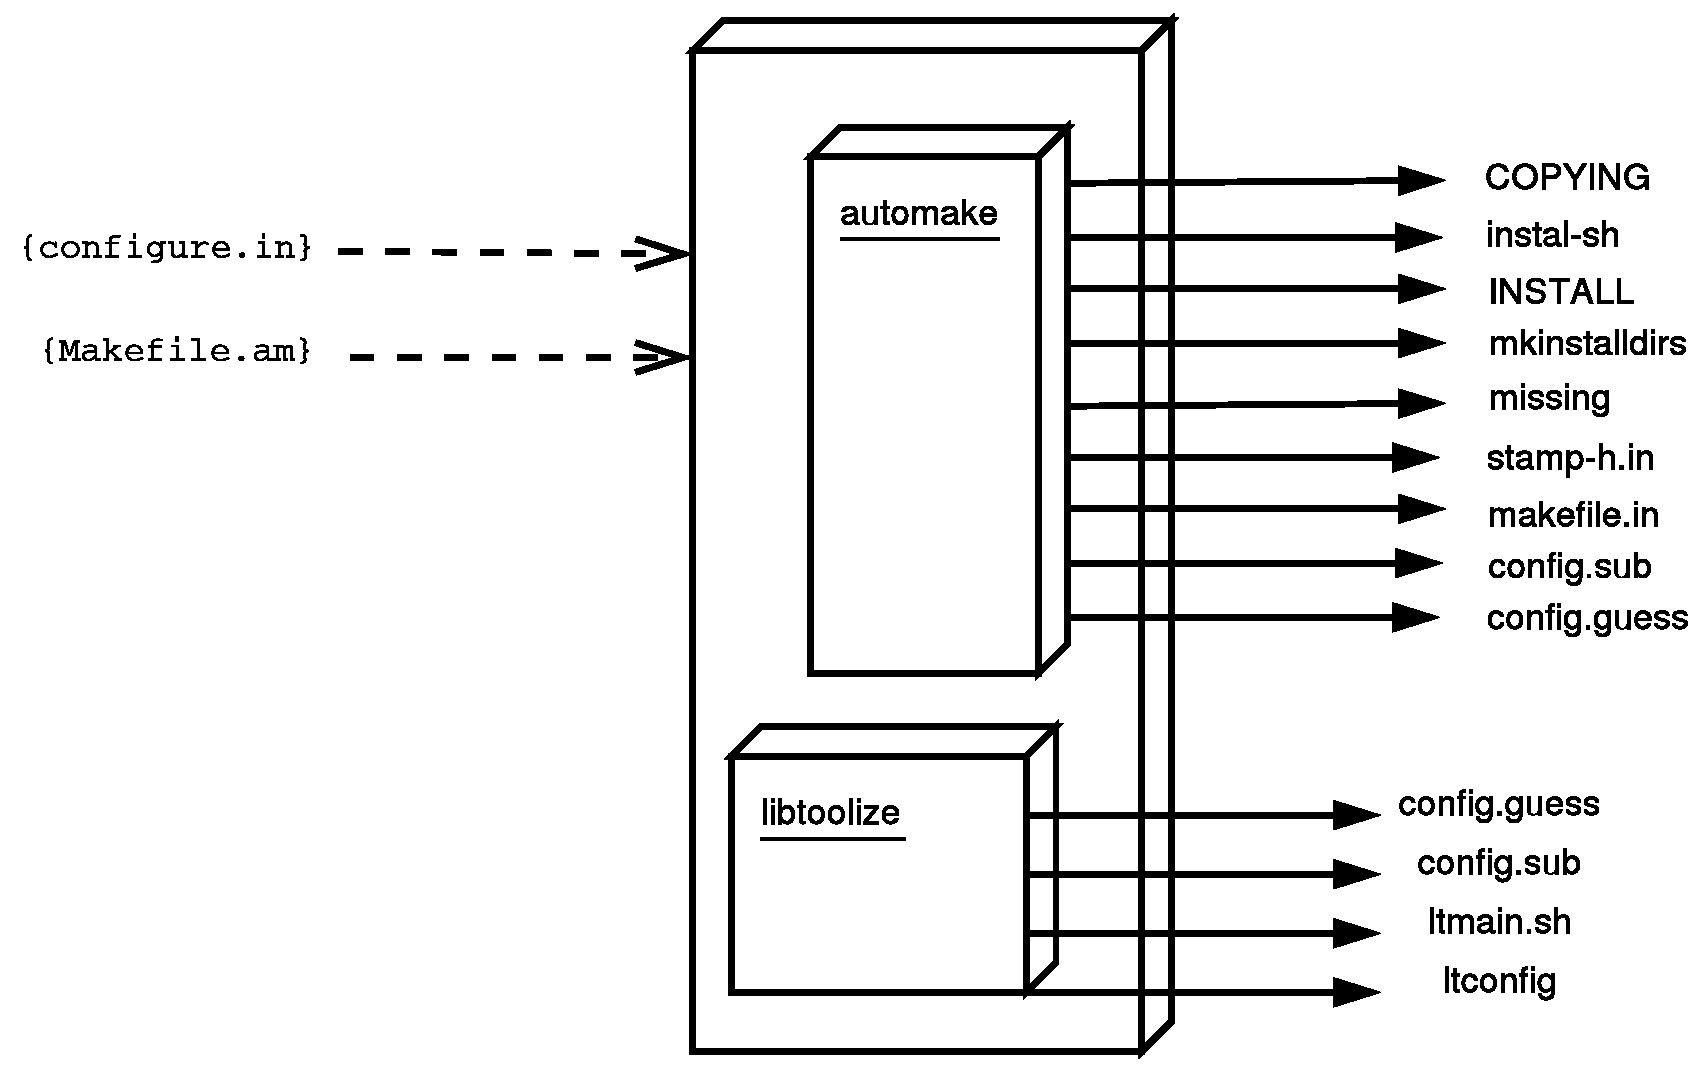
\includegraphics[scale=.35]{fig/DiagrammeAutomakeLibtoolize}
\end{center}

The versions of `config.guess' and `config.sub' installed differ between 
releases of Automake and Libtool, and might be different depending on whether 
libtoolize is used to install them or not. Before releasing your own package 
you should get the latest versions of these files from ftp://ftp.gnu.org/gnu/config,
in case there have been changes since releases of the GNU Autotools.
Currently, DIET is developped with, at least, libtool 1.4.3, automake 1.7.3 and 
autoconf 2.57. Bootstraping and compiling may succeed with others previous autotools version
but it is not garanteed.
%\footnote{Automake {\url{http://www.gnu.org/software/automake/automake.html}}}
%\footnote{Libtool {\url{http://www.gnu.org/software/libtool/libtool.html}}}


\subsection{autoconf}
autoconf\footnote{Autoconf {\url{http://www.gnu.org/software/autoconf/}}} expands the m4 macros in `configure.in', using macro 
definitions from `aclocal.m4', to generate the configure script.
\begin{center}
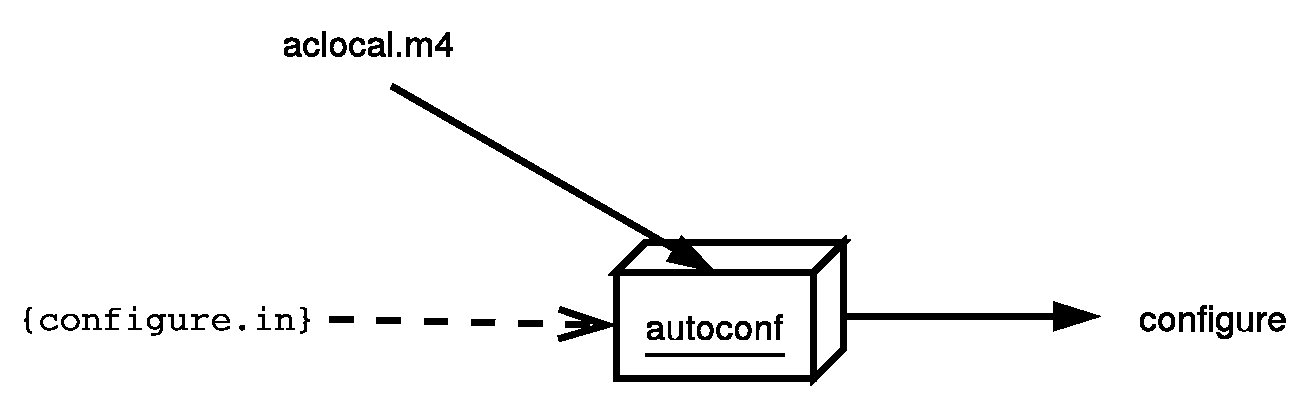
\includegraphics[scale=.35]{fig/DiagrammeAutoconf}
\end{center}
%\footnote{Autoconf {\url{http://www.gnu.org/software/autoconf/}}}

\subsection{configure}
The purpose of the preceding processes was to create the input files necessary
for configure to run correctly. You would ship your project with the generated
script and the files in columns, other input and processes (except 
`config.cache'), but configure is designed to be run by the person installing
your package. Naturally, you will run it too while you develop your project,
but the files it produces are specific to your development machine, and are
not shipped with your package -- the person installing it later will run 
configure and generate output files specific to their own machine.

Running the configure script on the build host executes the various tests 
originally specified by the `configure.in' file, and then creates another script,
`config.status'. This new script generates the `DIET\_config.h' header file from 
`DIET\_config.h.in', and `Makefile's from the named `Makefile.in's. Once 
`config.status' has been created, it can be executed by itself to regenerate
files without rerunning all the tests. Additionally, `AC\_PROG\_LIBTOOL'
was used, so ltconfig is used to generate a libtool script. 

\begin{center}
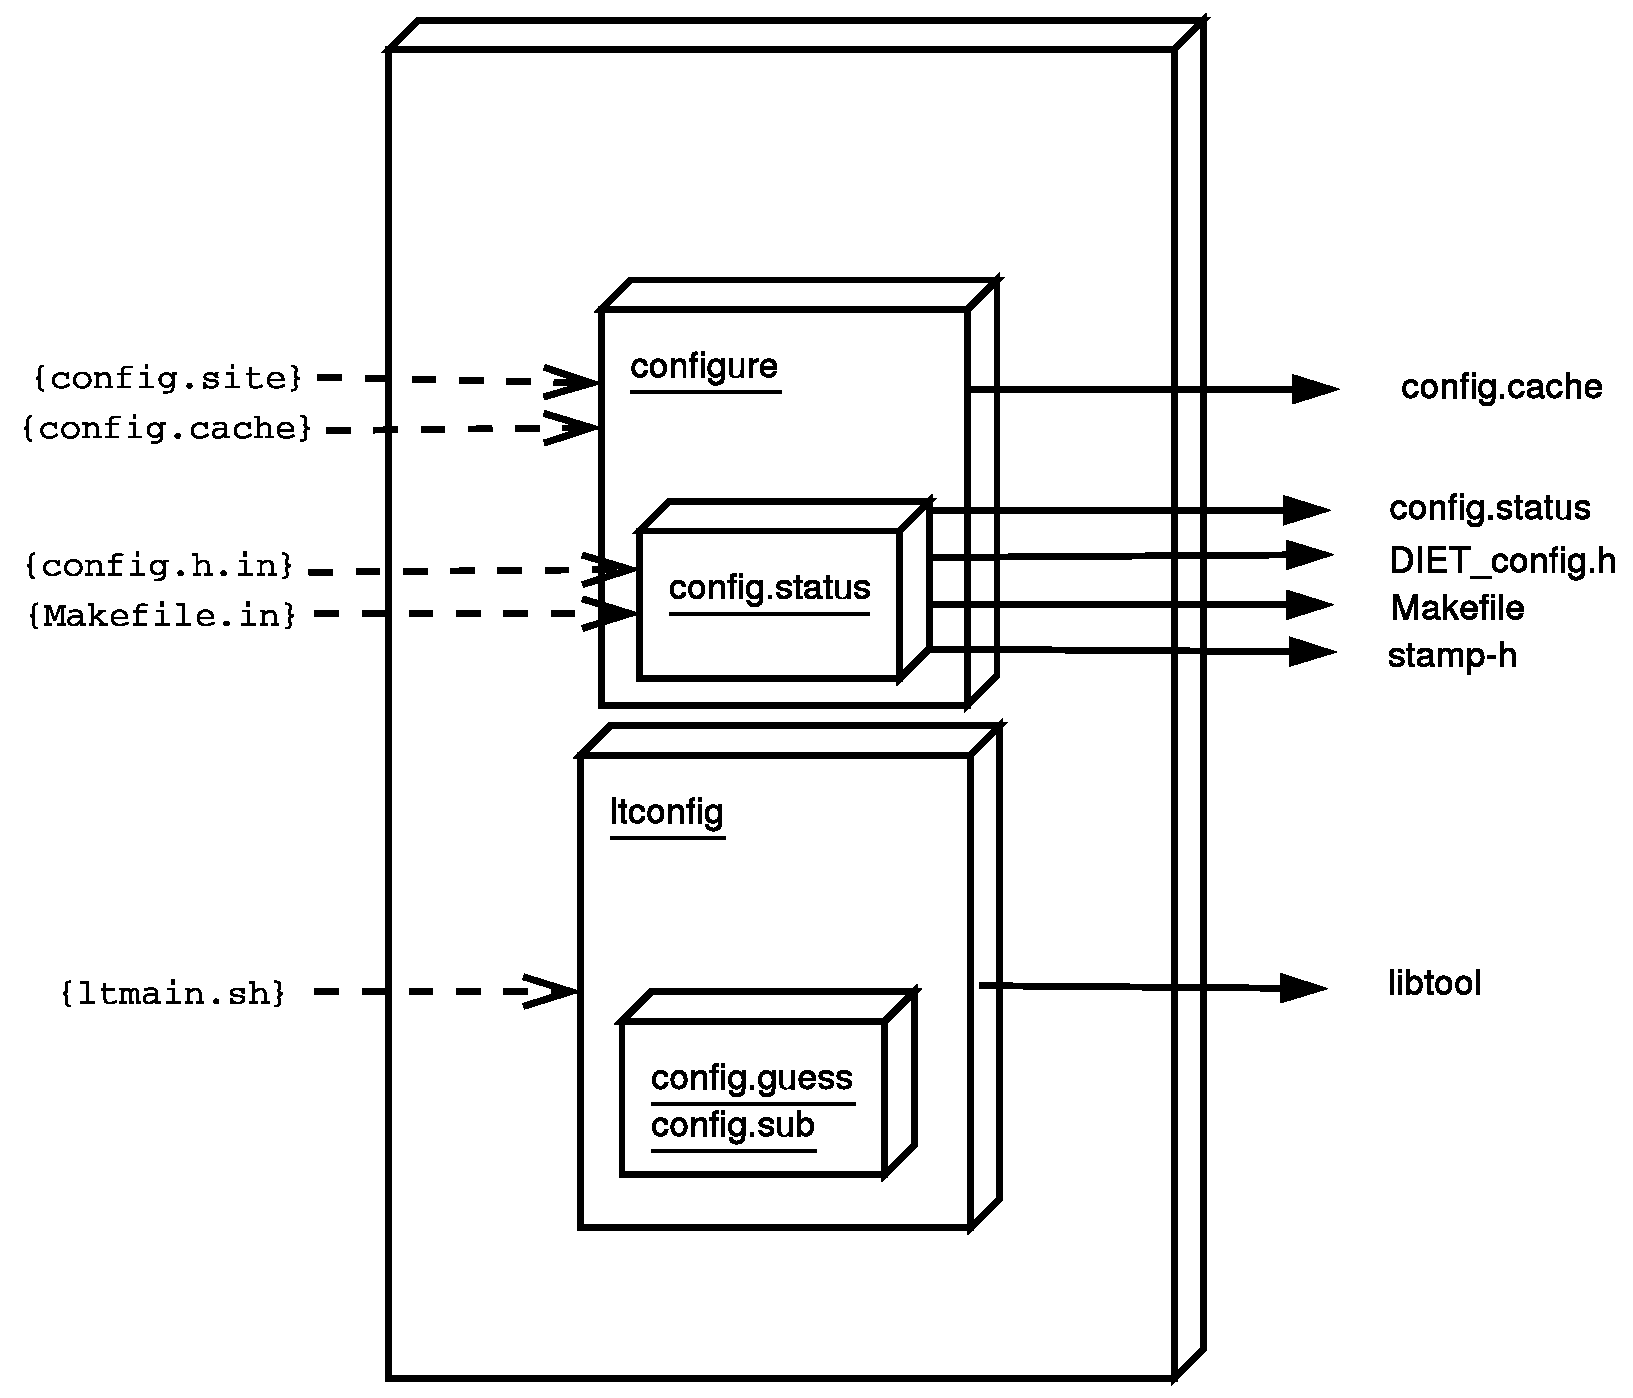
\includegraphics[scale=.35]{fig/DiagrammeConfigure}
\end{center}

\section{CORBA and asynchronism}
Datas from the book "Advanced CORBA Programming with C++""
\footnote{"Advanced CORBA Programming with C++"  from Michi Henning, Steve Vinoski} and
from omniORB\footnote{OMNIORB {\url{http://www.uk.research.att.com/omniORB/}}}
and from TAO\footnote{TAO {\url{http://www.cs.wustl.edu/~schmidt/TAO.html}}
}



%%%%
% Reference 
%%%%


\
\end{document}

